\section{Our Approach}

\begin{figure*}[t]
    \centering
    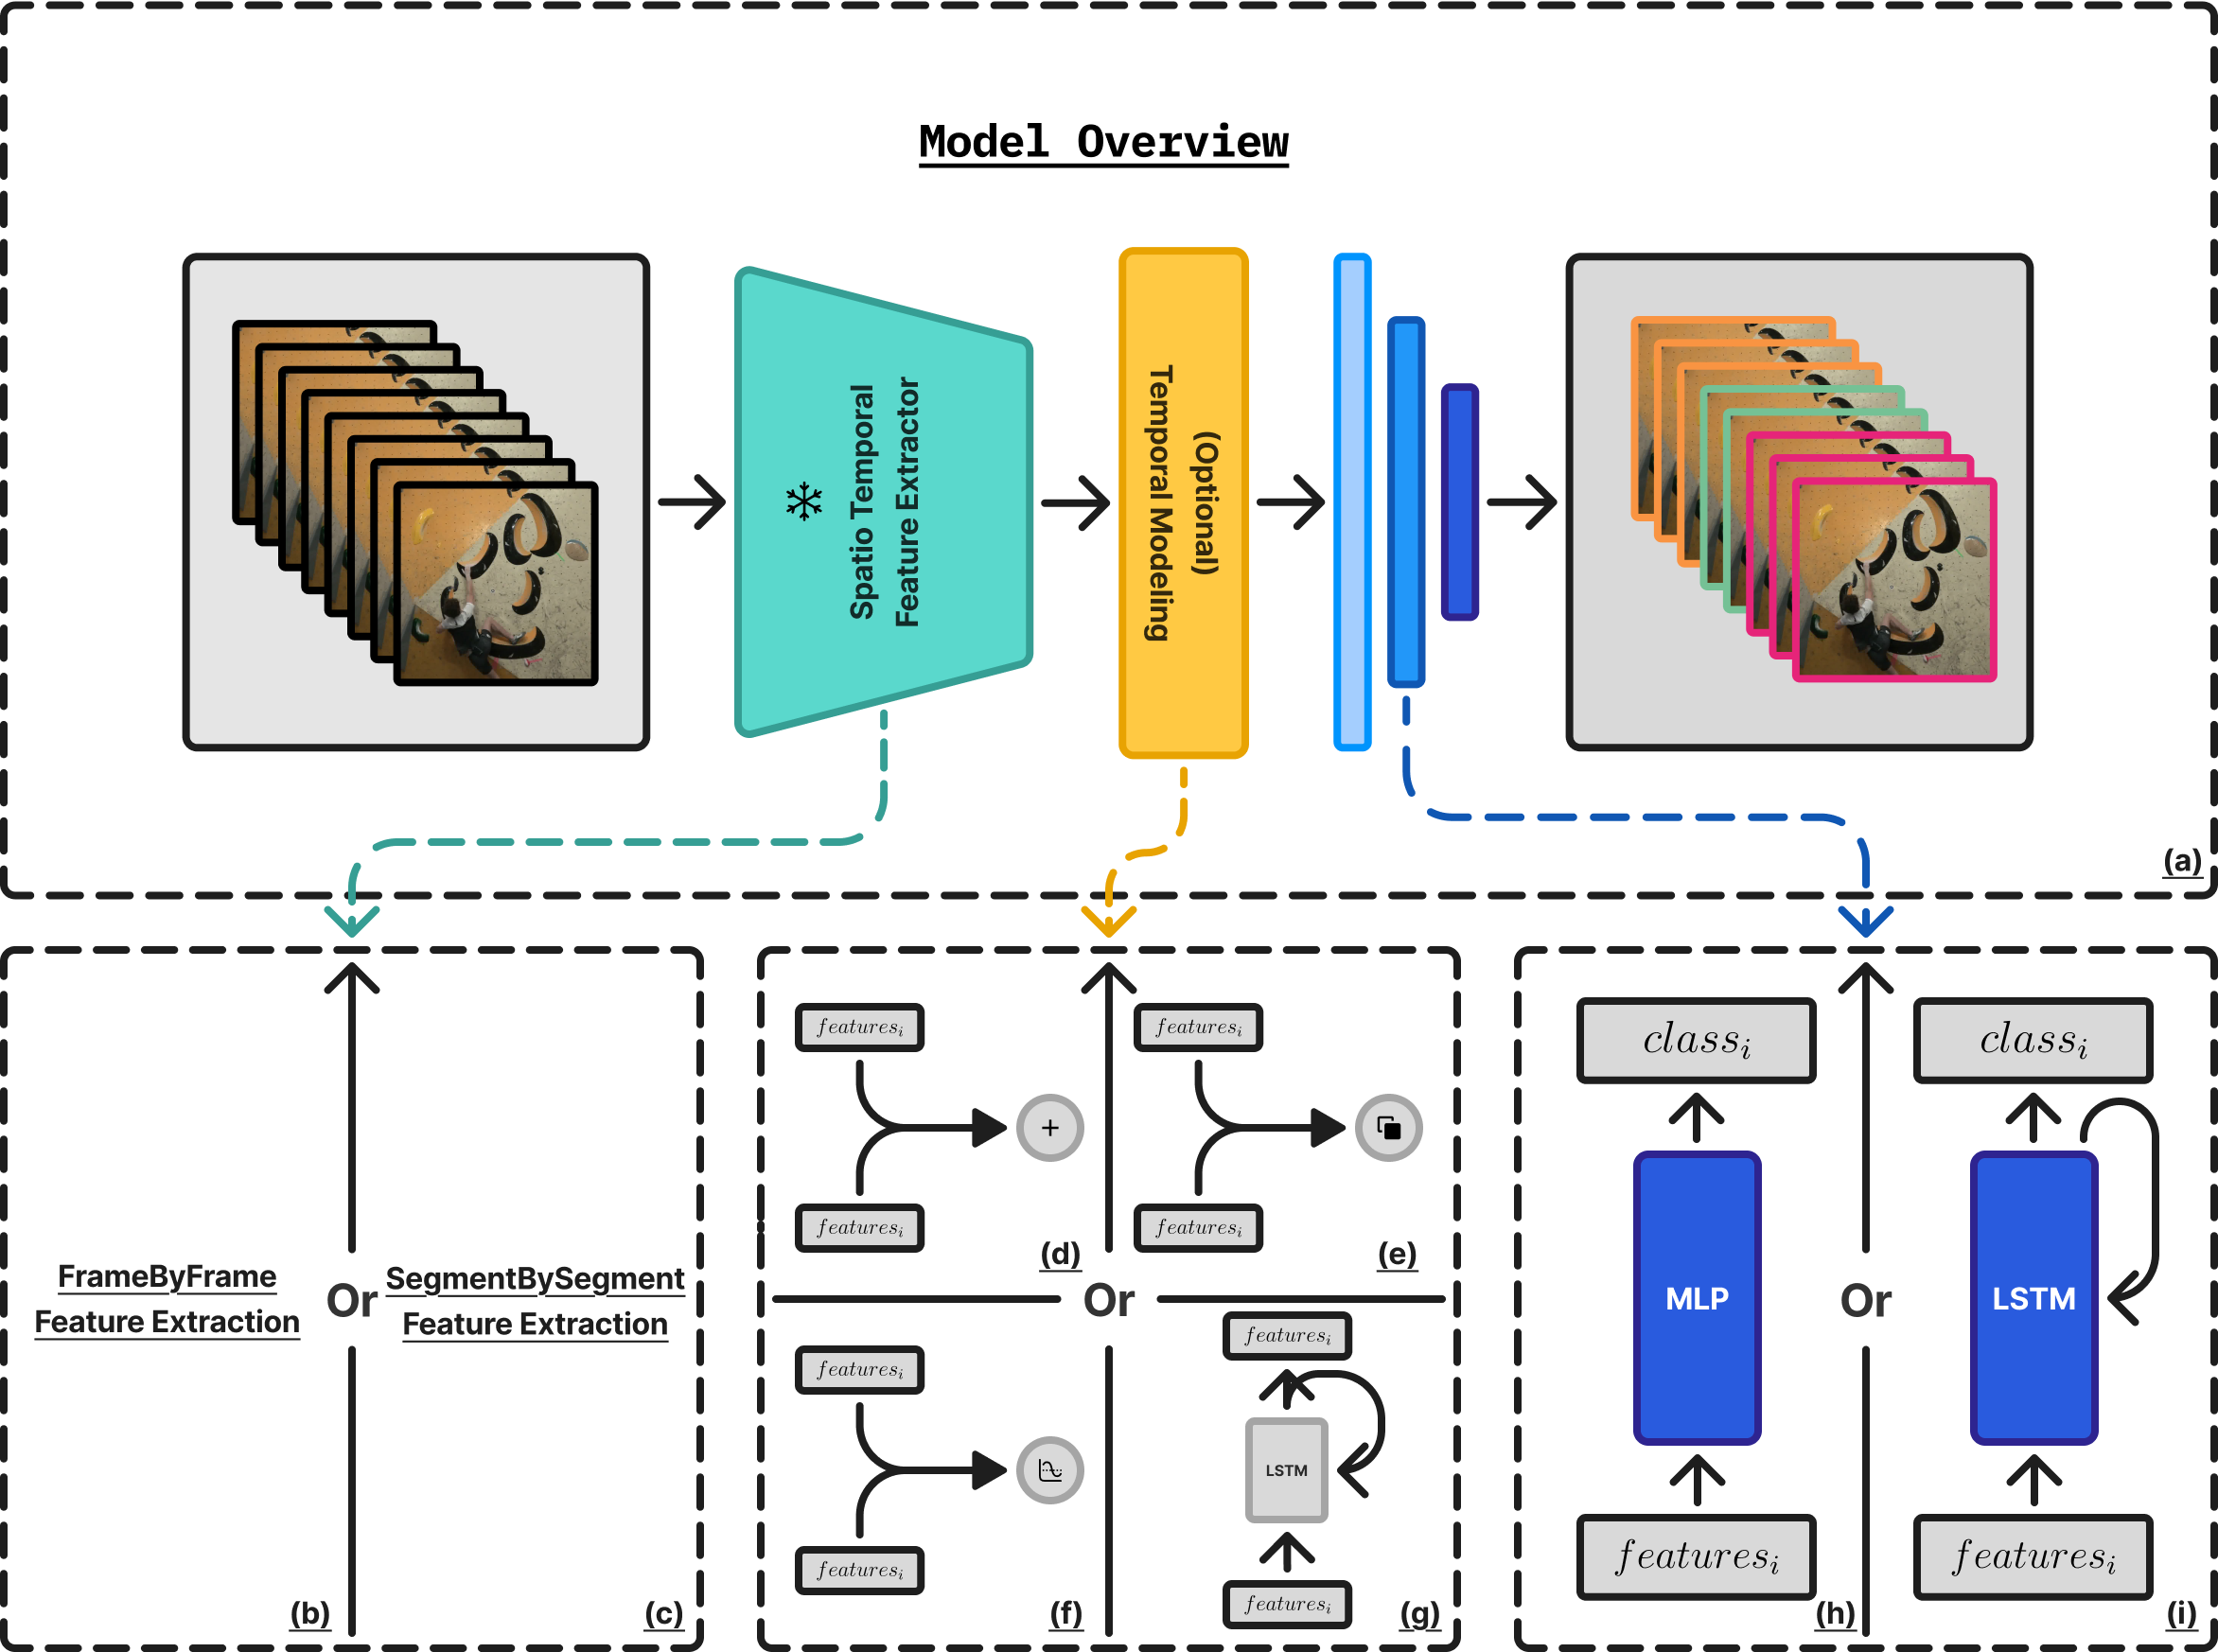
\includegraphics[width=\textwidth]{../../assets/figures/model-overview.png}
    \caption{Model Architecture Overview.}
    \label{fig:your-label}
\end{figure*}

Given the dataset size constraint, training a neural network from scratch with our data is infeasible and unlikely to yield meaningful results. To address this, we leverage pre-trained networks trained on large-scale datasets that contain similar types of actions to those found in our data. These actions are broad, non-atomic, and not highly granular, making them comparable to activities present in popular datasets like Kinetics.

Our strategy involves utilizing these pre-trained networks to extract feature representations from our videos, clips, and frames. Specifically, we extract features from the hidden layers of these networks — typically the layer immediately preceding the final classification layer — as they encode rich spatio-temporal information relevant to our task. These extracted features are then fed into a custom network designed for classification on our custom action labels.

This approach addresses multiple constraints simultaneously. First, it mitigates the impact of our limited dataset by capitalizing on robust features learned from extensive pre-training. Second, it reduces the computational burden, as we avoid the costly process of training a deep network from scratch. Finally, this method is well-suited to our project timeline, as designing and training a complex architecture would exceed our allocated 120 hours.

In the following sections, we describe the key components of our approach and how we train it.

\subsection{Spatio-Temporal Feature Extractors}
The backbone of our model is a spatio-temporal feature extractor designed to capture both spatial and temporal information from video data. We employ pre-trained models for this component, freezing their weights to retain the learned representations.

Two types of models are explored for this purpose: frame-level feature extractors and segment-level feature extractors.

\subsubsection{Frame-Level Extractors}
Frame-level extractors process individual frames independently to extract spatial features. Examples include 2D CNNs such as ResNet, vision transformers like DINO, CLIP, or ViT, and potentially handcrafted features such as object presence (e.g., brushes) or positional key points.

While handcrafted features can be informative, they introduce biases and require additional training for object detection, which is resource-intensive. Thus, our approach prioritizes automated feature extractors to maximize efficiency and robustness.

Once frame-level features are extracted, we explore several strategies to aggregate these features into a single representation for each video segment:

\noindent\textbf{\small{Averaging.}} The most common method, recommended in the literature for its simplicity and effectiveness.  
\noindent\textbf{\small{Addition.}} Similar to averaging but involves summing the features directly.  
\noindent\textbf{\small{Concatenation.}} Combines frame features without additional operations.  
\noindent\textbf{\small{Temporal Modeling.}} Uses models like LSTMs or Transformers to capture temporal dependencies, offering improved contextual understanding at the cost of higher computational complexity.

\subsubsection{Segment-Level Extractors}
Segment-level extractors process multiple consecutive frames directly, capturing both spatial and temporal patterns. Examples include 3D CNNs, which extend 2D CNN architectures to model motion and temporal dynamics, and transformer-based models that have demonstrated strong performance on video tasks. While effective, these models are typically more computationally demanding.

\subsection{Temporal Sub-Sampling}
To improve efficiency without sacrificing performance, we incorporate temporal sub-sampling. This technique involves reducing the frame rate before feature extraction, as consecutive frames in bouldering videos often exhibit minimal visual change. Studies in the field highlight that temporal sub-sampling is a simple yet highly effective method for reducing computational load without significant performance degradation.

\subsection{Temporal Context Window}
The temporal context window defines the number of consecutive frames the model processes at once. Choosing an optimal window size is crucial:

\noindent\textbf{\small{Short Window.}}
It may not capture sufficient context for accurate classification.

\noindent\textbf{\small{Long Window.}}
It risks embedding the entire video into a single feature, increasing computational costs and reducing model flexibility.

As the temporal context window of the backbone networks is quite limited to around 16-32 frames usually, processing the whole 4 minutes of video and extracting a single feature for the entire video is both computationally costly and not practical in our case. This would be more practical for video classification tasks, where the goal is to classify the whole video. In our case, we aim to extract different time segments and classify them individually. This is why we present two approaches for processing these time segments.

Balancing these factors is key to achieving optimal performance.

By combining pre-trained feature extractors, temporal sub-sampling, and thoughtful hyperparameter tuning, our approach aims to achieve robust performance despite dataset limitations.

\subsection{Classifier}

This is the component of our network that'll receive the spatio temporal features corresponding to a video segment / clip and output the class of the action that is being performed in this segment.

For this we consider two approaches, the first one is to use a simple MLP with a single hidden layer and the second one is to use an LSTM with a single layer. The idea behind the use of the LSTM is that it can capture the temporal dependencies between the frames / segments and thus potentially improve the model's performance.

We could also use an attention mechanism to allow the model to focus on the most important frames / segments but this would increase the model's complexity and thus the training time and the computational cost.

Another possible improvement would be to use fixed or learnable positional embeddings in combination with the MLP in order to incorporate temporal awareness into the MLP. 

%  --- --- ---

\subsection{Training Methodology}

\subsubsection*{Backbone Model}
We experimented with several backbone models for feature extraction, leveraging both frame-level and segment-level networks. Notable examples include:

\noindent\textbf{\small{DINO}} and \noindent\textbf{\small{CLIP.}} Vision Transformers used as frame-level feature extractors for their strong spatial representation capabilities.

\noindent\textbf{\small{X3D}}, \noindent\textbf{\small{R3D}}, and \noindent\textbf{\small{Slowfast.}} Segment-level extractors known for their robust spatio-temporal modeling.

Most of the backbones we use are pre-trained or fine-tuned on the Kinetics dataset, except for CLIP, which leverages large-scale internet data.

\subsubsection*{Loss Function}
Our classification model is trained using the \textbf{cross-entropy loss} function, defined as:

\[
\mathcal{L} = -\sum_{i=1}^{N} y_i \log \hat{y}_i
\]

where \(y_i\) is the true label and \(\hat{y}_i\) is the predicted probability for class \(i\). While cross-entropy loss effectively handles multi-class classification, alternative losses such as focal loss or label-smoothing loss have been proposed in the literature to address class imbalance and calibration issues. These approaches may be worth exploring in future work.

\subsubsection*{Classifier Model}
\todo[inline]{Describe the architecture of the MLP and LSTM model that are going to be used for classification.}

\subsubsection*{Training Setup}
The training pipeline was configured as follows:

\noindent\textbf{Optimizer.} Adam optimizer with a learning rate of $1 \times 10^{-4}$.

\noindent\textbf{Batch Size.} 32 samples per batch for efficient convergence.

\noindent\textbf{Early Stopping.} Applied based on validation loss with a patience of 5 epochs to prevent overfitting.

\noindent\textbf{Batch Structure.} Each batch consists of video segments rather than entire videos. This approach ensures manageable memory usage and allows the model to learn from diverse temporal contexts within each batch.

To prevent data leakage during validation, we ensured that segments from the same video were never split across training and validation sets. This avoids the model unintentionally learning video-specific patterns rather than generalizable features.

\subsubsection*{Data Filtering and Preprocessing}
To improve data quality and enhance model performance, we applied several preprocessing steps:

\noindent\textbf{Removal of Personless Frames.} Frames without visible climbers were excluded to reduce noise.

\noindent\textbf{Cleaning of Low-Quality Data.} Unannotated frames were removed rather than assigning them a generic "nothing" label. This improved class balance and reduced label ambiguity.

\noindent\textbf{Stopwatch Class Removal.} We excluded segments showing only the competition timer, as these frames added no meaningful information to the model's predictions.

\begin{AIbox}{Python Package - Cached Dataset.}
    To accelerate training, we developed a custom Python package called \textbf{cached-dataset} - \href{https://github.com/raideno/video-dataset}{https://github.com/raideno/video-dataset}. This tool caches the transformation of a dataset to disk, significantly reducing data loading overhead during training and feature extraction. This allow us to efficiently iterate through training experiments and hyperparameter tuning.
\end{AIbox}

By combining robust pre-trained feature extractors, temporal sub-sampling, and thoughtful data filtering strategies, our training methodology effectively addresses the challenges posed by our limited dataset. These strategies ensured a stable and efficient training process while maximizing model performance.